\subsection{SP-25 (PSI)}
Transportni vrstva, protokol TCP, spolehlivost doručení paketů, zahlcení, srovnání s protokolem UDP. Překlad síťových adres (NAT) na síťové a transportní vrstvě. Systém doménových jmen (DNS).

\subsubsection*{Transportní vrstva}
\begin{itemize}
	\item zajišťuje doručení dat konkrétním aplikacím (přidává k IP adrese ještě port)
	\item řeší spolehlivost dodání dat
	\begin{itemize}
		\item možnost stop and wait --- jednoduchá, ale neefektivní, doručuje data přesně v pořadí jak jdou za sebou
		\item možnost stop and go --- nezajistí, že data dorazí do cíle, přijímač posílá vysílači stop a go signály
		\item sliding window --- okénko o nějaké velikosti, první se odesílá, na poslední se čeká na ACK
	\end{itemize}
\end{itemize}

\subsubsection*{TCP}
\begin{itemize}
	\item nejznámější protokol transportní vrstvy, který zajišťuje spolehlivé doručení dat
	\item garantuje jak doručení, tak pořadí paketů
	\item je duplexní, obě strany jsou vysílačem i přijímačem
	\item navazování a ukončování spojení:	
	
	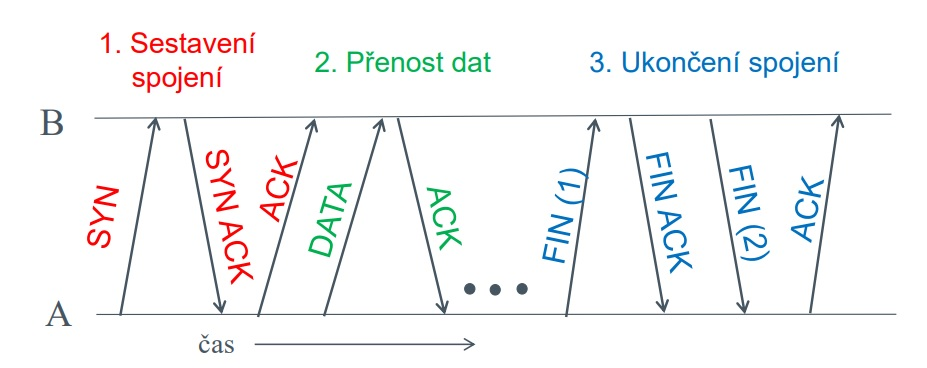
\includegraphics[width=0.8\textwidth]{img/SP-25_0.jpg}
	
	\item struktura TCP paketu
	
	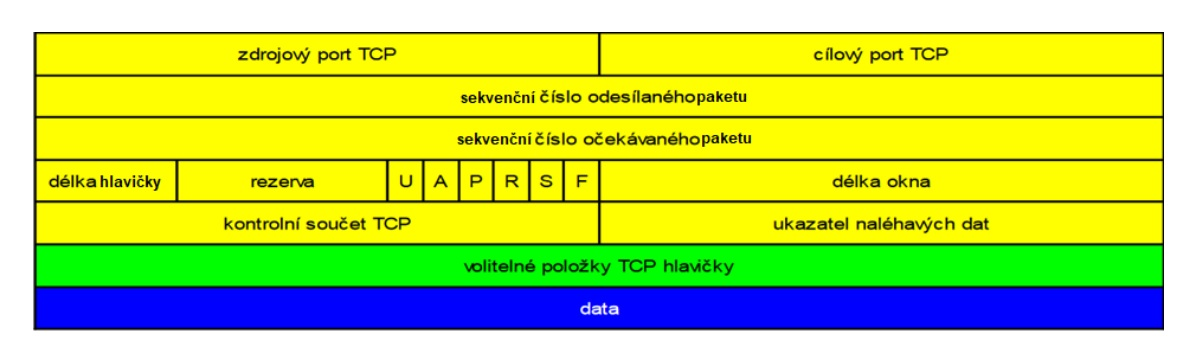
\includegraphics[width=0.8\textwidth]{img/SP-25_1.jpg}
	
	\item pro řízení toku se používá mechanismus klouzavého okénka (sliding window) --- přijímač nastavuje délku okénka dle svých možností
	
	\item vysílač ještě musí nějak zajistit, aby se nepřetížila linka, to je složitější a liší se to dle varianty TCP --- nastavuje se CWL (congestion window length)
	\item některé druhy obnovují rychlost (velikost CWL) po výpadku rychleji, jiné pomaleji
	
	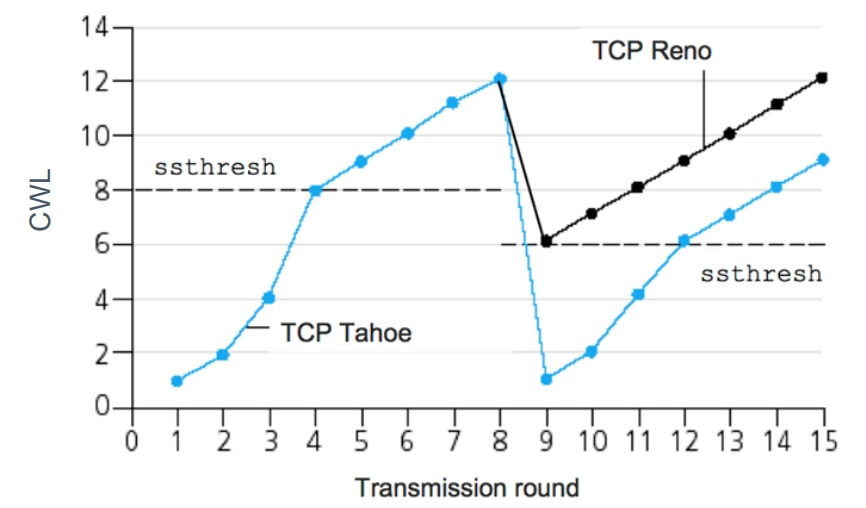
\includegraphics[width=0.6\textwidth]{img/SP-25_2.jpg}
	
\end{itemize}

\subsubsection*{UDP}
\begin{itemize}
	\item nižší režie --- vyšší propustnost než TCP
	\item běžně se používá na přenos hlasu či videa
	\item struktura UDP paketu:
	
	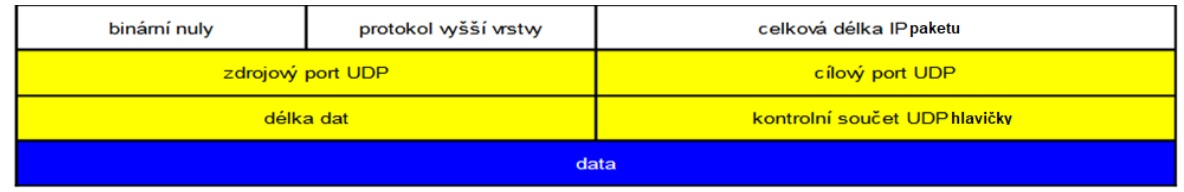
\includegraphics[width=0.8\textwidth]{img/SP-25_3.jpg}
\end{itemize}

\subsubsection*{NAT}
\begin{itemize}
	\item díky transportní vrstvě a portům je možné na routeru překládat IP adresy pro více spojení a stanic za routerem
	\item směrem ven se přeloží IP adresa, pokud je to nutné tak i port
	\item tím se vytvoří mapování na routeru --- tento výstupní port je mapován ke konkrétní IP a portu za routerem
	\item při odpovědi se dle portu rozhodne na jakou IP (a port) data poslat
\end{itemize}

\subsubsection*{DNS}
\begin{itemize}
	\item IP adresy jsou špatně zapamatovatelné
	\item DNS --- Domain Name System je primárně určen k překladu doménových jmen na IP adresy a naopak
	\item DNS je hierarchický a nezabezpečený
	\item DNS je zásadní i pro další služby jako email
	\item běží typicky na portu 53 a většina implementací využívá UDP
	
	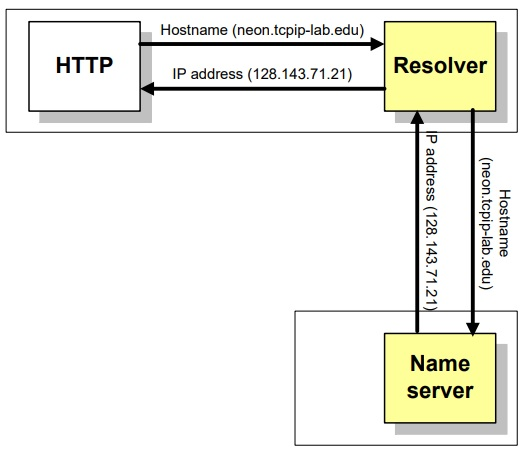
\includegraphics[width=0.5\textwidth]{img/SP-25_4.jpg}
	
	\item hierarchie domén:
	
	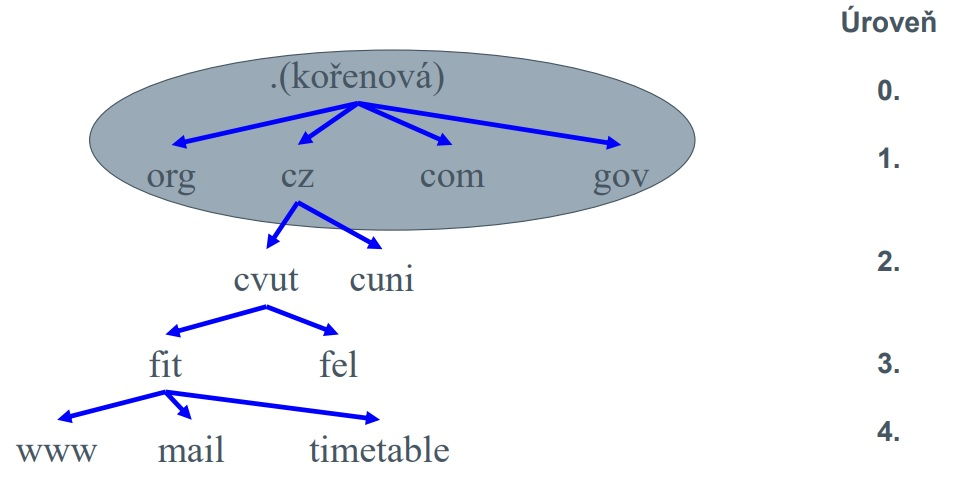
\includegraphics[width=0.7\textwidth]{img/SP-25_5.jpg}
	
	\item 4 typy Top Level Domains (TLD) (1. úrovně)
	\begin{itemize}
		\item Generic TLD (gTLD) --- 3 znaky označující funkci organizace (gov, mil, edu, org, com, net)
		\item Country Code TLD --- 2 znaky označující zemi (cz, us, de, eu)
		\item New Generic TLD --- libovolný řetězec (max 63 znaků)
		\item reverzní doména --- in-addr.arpa
	\end{itemize}
	\item dříve centralizovaný systém všech domén v souboru hosts.txt
	\item existuje iterativní způsob dotazování (dotaz lokálnímu DNS serveru, ten se postupně od root zeptá všech nutných dalších DNS serverů) nebo rekurzivní (zeptají se v řadě za sebou, lokální rootu, root TLD atd atd)
	\item existuje DNSSEC --- zabezpečený DNS (přes asymetrickou kryptografii)
	\item existuje dynamické DNS (DynDNS) --- pro případ zařízení, která často mění IP adresu
\end{itemize}